\documentclass[11pt, a4paper]{article}
%\usepackage{proj1}
\usepackage{natbib}
\usepackage{fancyhdr}  
\usepackage{subcaption}
\usepackage{caption}
\usepackage{graphicx}
\usepackage{numprint}
\usepackage{multirow}
\linespread{1.25} 
\setlength{\parindent}{0cm}
\graphicspath{{Images/}}
\usepackage{hyperref}
\usepackage{amsmath}
\usepackage{amsfonts}
\usepackage{amssymb}
\usepackage{amsthm}
\usepackage{mathtools}
\usepackage{commath}
\usepackage{bbm}

%\usepackage[sc,osf]{mathpazo}
\usepackage{subcaption}
\usepackage[a4paper, top=1in, left=1.0in, right=1.0in, bottom=1in, includehead, includefoot]{geometry} %Usually have top as 1in

\usepackage{listings}
\usepackage{color} %red, green, blue, yellow, cyan, magenta, black, white
\definecolor{mygreen}{RGB}{28,172,0} % color values Red, Green, Blue
\definecolor{mylilas}{RGB}{170,55,241}


\hypersetup{colorlinks,linkcolor={black},citecolor={blue},urlcolor={black}}
\usepackage{color}
\urlstyle{same}


\theoremstyle{definition}
\newtheorem{definition}{Definition}[section]

\newcommand{\adja}{q_a}
\newcommand{\adjb}{q_b}
\newcommand{\adjaB}{q_{a,\partial \Omega}}
\newcommand{\adjbB}{q_{b,\partial \Omega}}
\newcommand{\adjB}{q_{\partial \Omega}}
\newcommand{\Adja}{\mathbf{p}}
\newcommand{\Adjb}{q}
\newcommand{\adj}{q}
\newcommand{\Adjc}{{q}_{\partial \Omega}}
\newcommand{\ra}{\rho_a}
\newcommand{\rb}{\rho_b}
\newcommand{\w}{\mathbf{w}}
\newcommand{\f}{\mathbf{f}}
\newcommand{\ve}{\mathbf{v}}
\newcommand{\n}{\mathbf{n}}
\newcommand{\h}{\mathbf{h}}
\newcommand{\K}{\mathbf{K}}
\newcommand{\hr}{\widehat \rho}
\newcommand{\jf}{\mathbf j}

%	\begin{figure}[h]
%		\centering
%		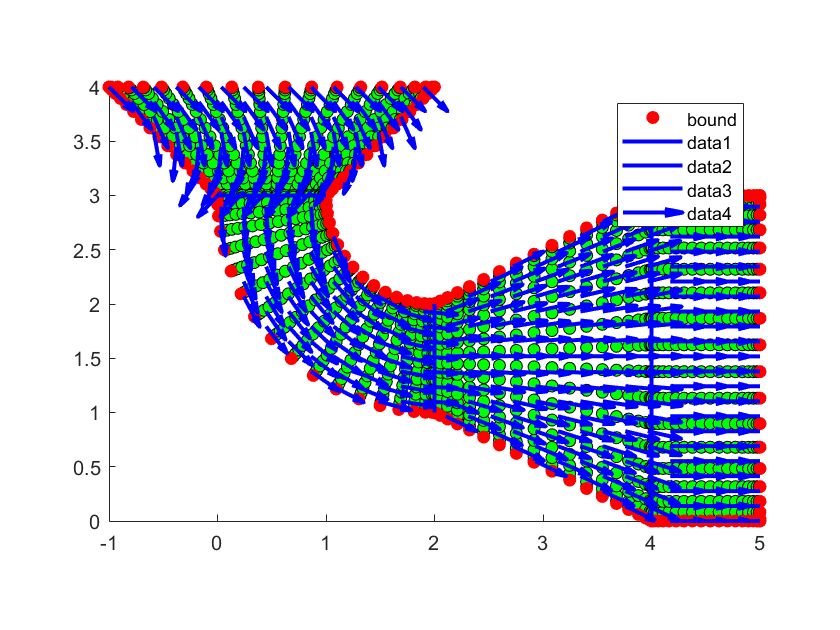
\includegraphics[scale=0.35]{F1.png}
%		\caption{Forward $\rho$ for $a = 0.01$} 
%		\label{F1}
%	\end{figure}

\begin{document}

\section{Validation Tests}
\subsection{Exact Tests}
Several examples are run, using exact solutions, to validate the multishape code. This is done using an exact solution to the advection diffusion equation on an infinite domain, so that Dirichlet boundary conditions, matching the value of the exact solution on the boundary of the multishape, can be applied.
The exact solution is \cite{Hutomo_2019}
\begin{align*}
	\rho &= \exp(\alpha t + \beta_1 y_1 + \beta_2 y_2)\\
	\mathbf v &= \left(\beta_1 - \frac{\alpha}{2 \beta_1} + p_1\exp(-\beta_1 y_1) , \beta_2 - \frac{\alpha}{2 \beta_2} + p_2\exp(-\beta_2 y_2) \right),
\end{align*}
where $\beta_1 = 0.1$, $\beta_2 = 0.1$, $\alpha = -0.5$, $p_1 = -1$ and $p_2 = 1$.
We compare the exact solution on a box of dimensions $[0,2] \times [0,2] $ with different discretizations of the box using multishape, see Figure \ref{F2}. Each of the shapes are discretized with $N = 20$ and $N = 30$ points in each spatial direction, which means that the dissected box has more points in total than the original box. The ODE solver tolerances are $10^{-9}$. The solution can be seen in Figure \ref{F3}. The question is whether the results of the PDE on the box and the different discretizations of the box have a similar error when compared to the exact solution. The absolute and relative errors are measured in an $L_2$ norm in space and an $L_\infty$ norm in time and are displayed in Table \ref{Tab1:ErrorsExBox}. The leftmost column contains errors for the non-rectangular quadrilateral, which is shown in Figure \ref{F3a}.
\begin{table}
	\caption{Errors compared to exact solution for different discretizations (into one, two and three shapes) of the box and a quadrilateral}
	\begin{tabular}{ ||c| c| c| c| c|c|| }
		\hline
		\hline
		 & One Shape & Two Shapes & Three Shapes & Four Shapes & Quadrilateral \\ 
		 \hline
		 Abs. E., $N =20$& $2.2063 \times 10^{-7}$ & $3.2073 \times 10^{-7}$ & $3.9108\times 10^{-7}$ & $3.902\times 10^{-7}$& $2.2844\times 10^{-7}$\\  
		 Rel. E., $N =20$& $1.1235 \times 10^{-9}$& $1.1377 \times 10^{-9}$ &$1.15 \times 10^{-9}$ &  $1.0026 \times 10^{-9}$& $1.116\times 10^{-9}$\\
		Abs. E., $N =30$& $2.1913 \times 10^{-7}$ & $3.1878 \times 10^{-7}$ & $3.8859\times 10^{-7}$ & $3.8767\times 10^{-7}$ & $2.2505\times 10^{-7}$\\  
		Rel. E., $N =30$ & $1.1159 \times 10^{-9}$& $1.1308 \times 10^{-9}$ &$1.1427\times 10^{-9}$ &  $9.9612 \times 10^{-10}$ & $1.0995\times 10^{-9}$  \\
		\hline
		\hline
	\end{tabular}
\label{Tab1:ErrorsExBox}
\end{table}

	\begin{figure}[h]
		\centering
		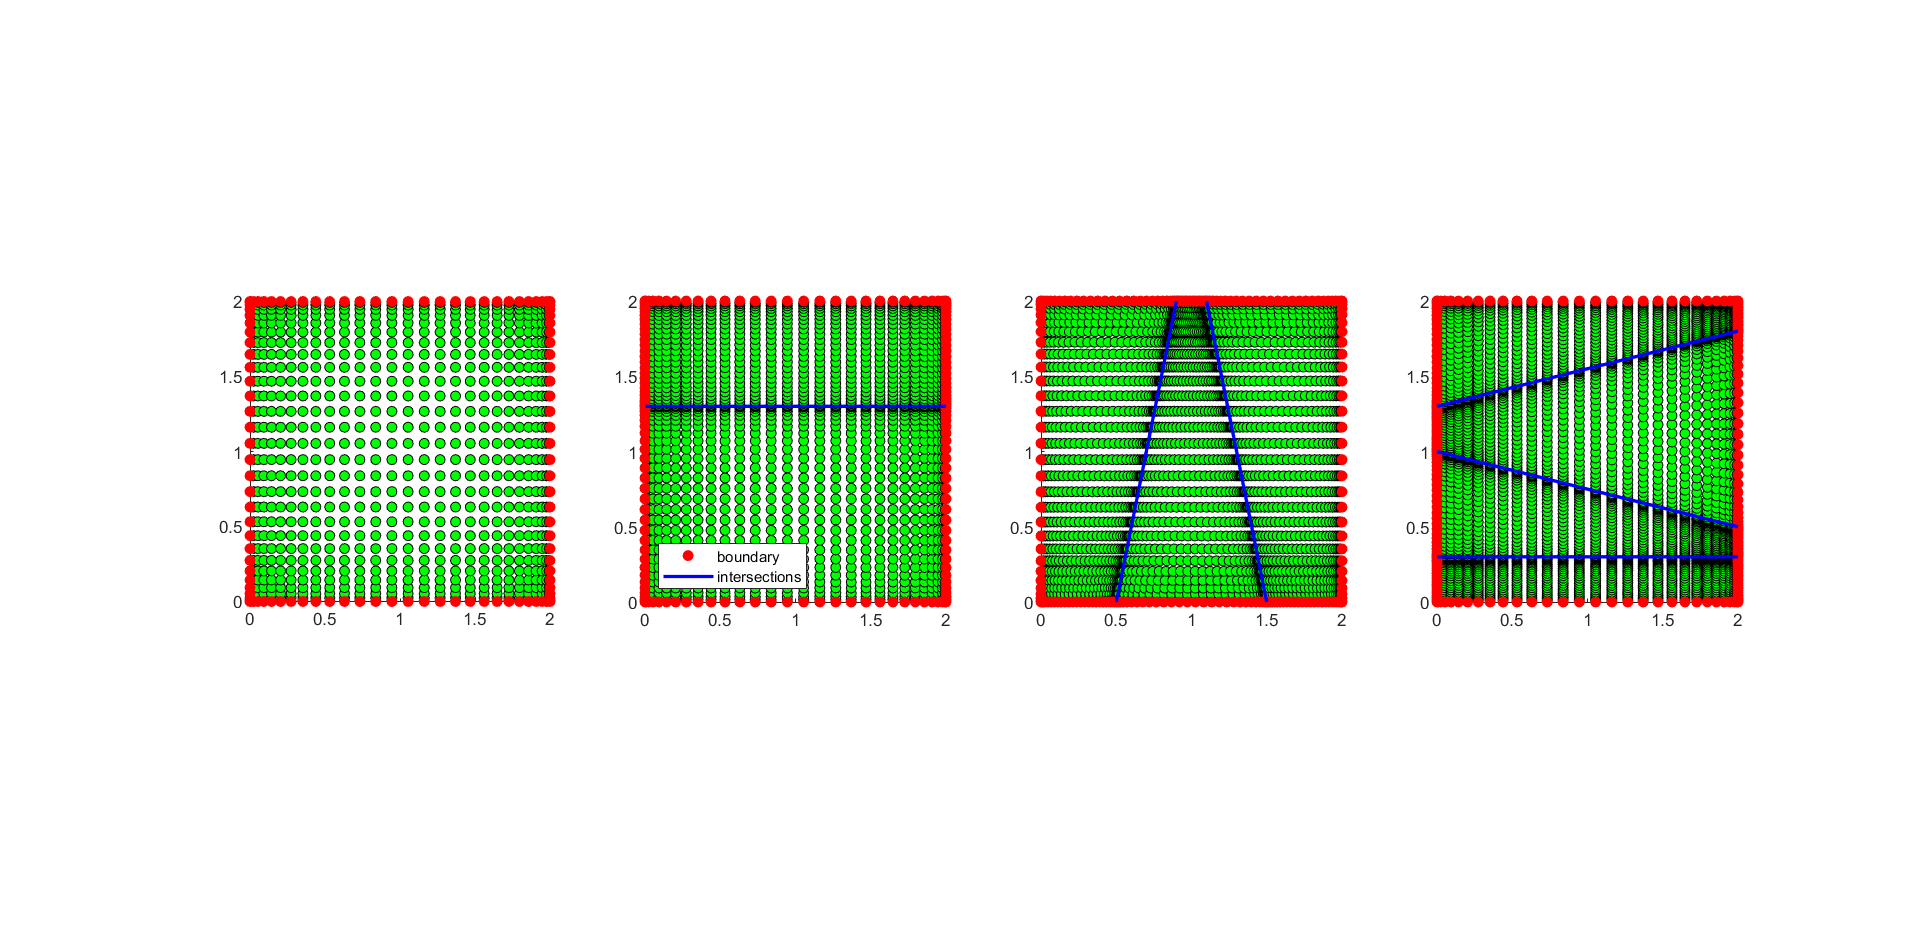
\includegraphics[scale=0.35]{BoxSections.png}
		\caption{Different discretizations of the box.} 
		\label{F2}
	\end{figure}

	\begin{figure}[h]
		\centering
		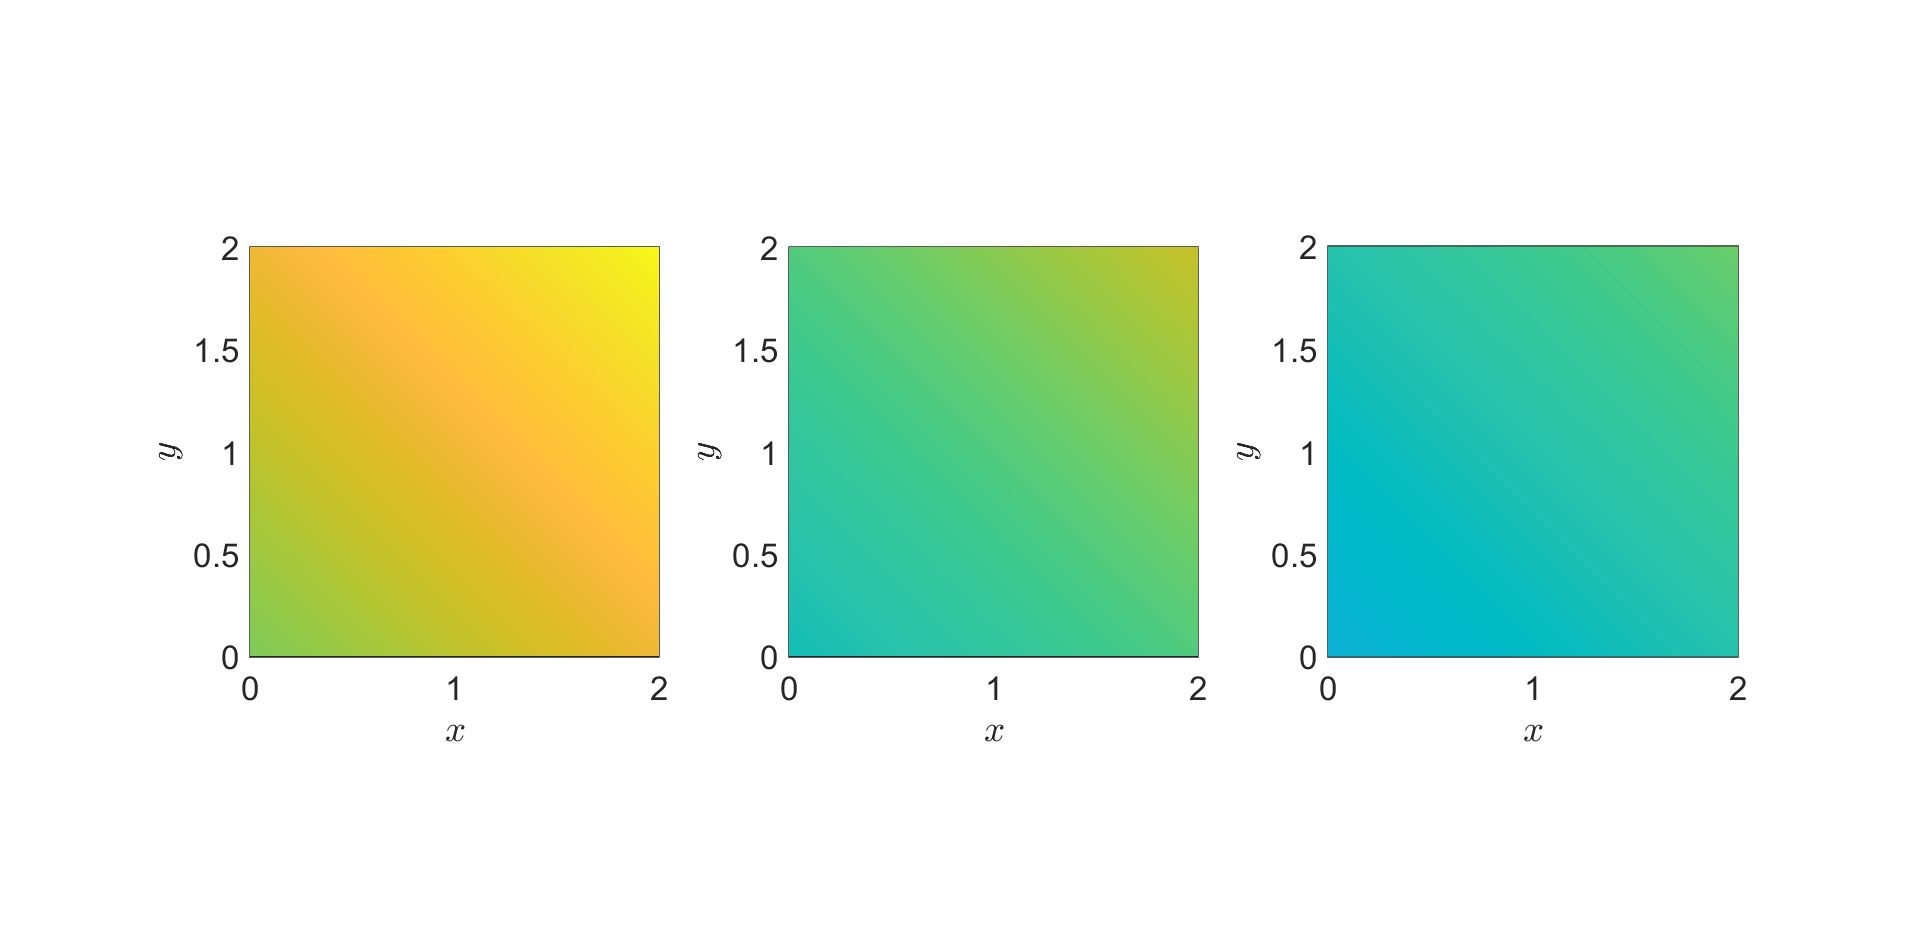
\includegraphics[scale=0.35]{boxEx.png}
		\caption{Exact solution on the box.} 
		\label{F3}
	\end{figure}
	\begin{figure}[h]
		\centering
		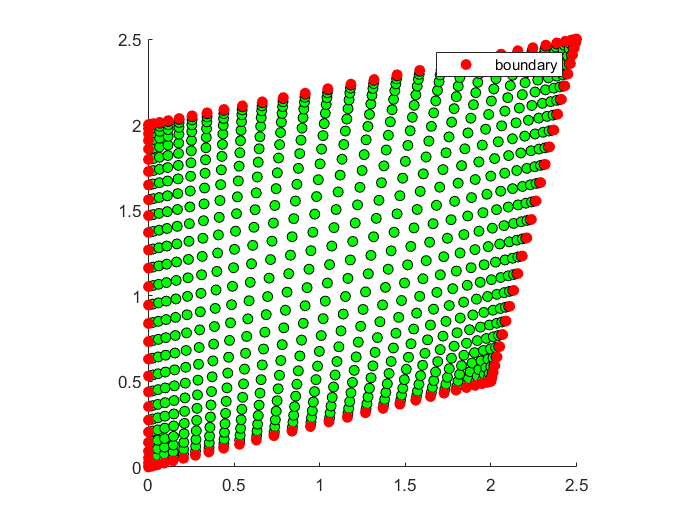
\includegraphics[scale=0.35]{quad.png}
		\caption{Quadrilateral domain.} 
		\label{F3a}
	\end{figure}

The same test can be done for a wedge. Here, a single wedge and discretized versions are considered, see Figure \ref{F4}. Table \ref{Tab2:ErrorsExWedge} shows the errors measured against the exact solution for different discretizations of the wedge for $N = 20$ and $N = 30$. The solution can be seen in Figure \ref{F5}.
\begin{figure}[h]
	\centering
	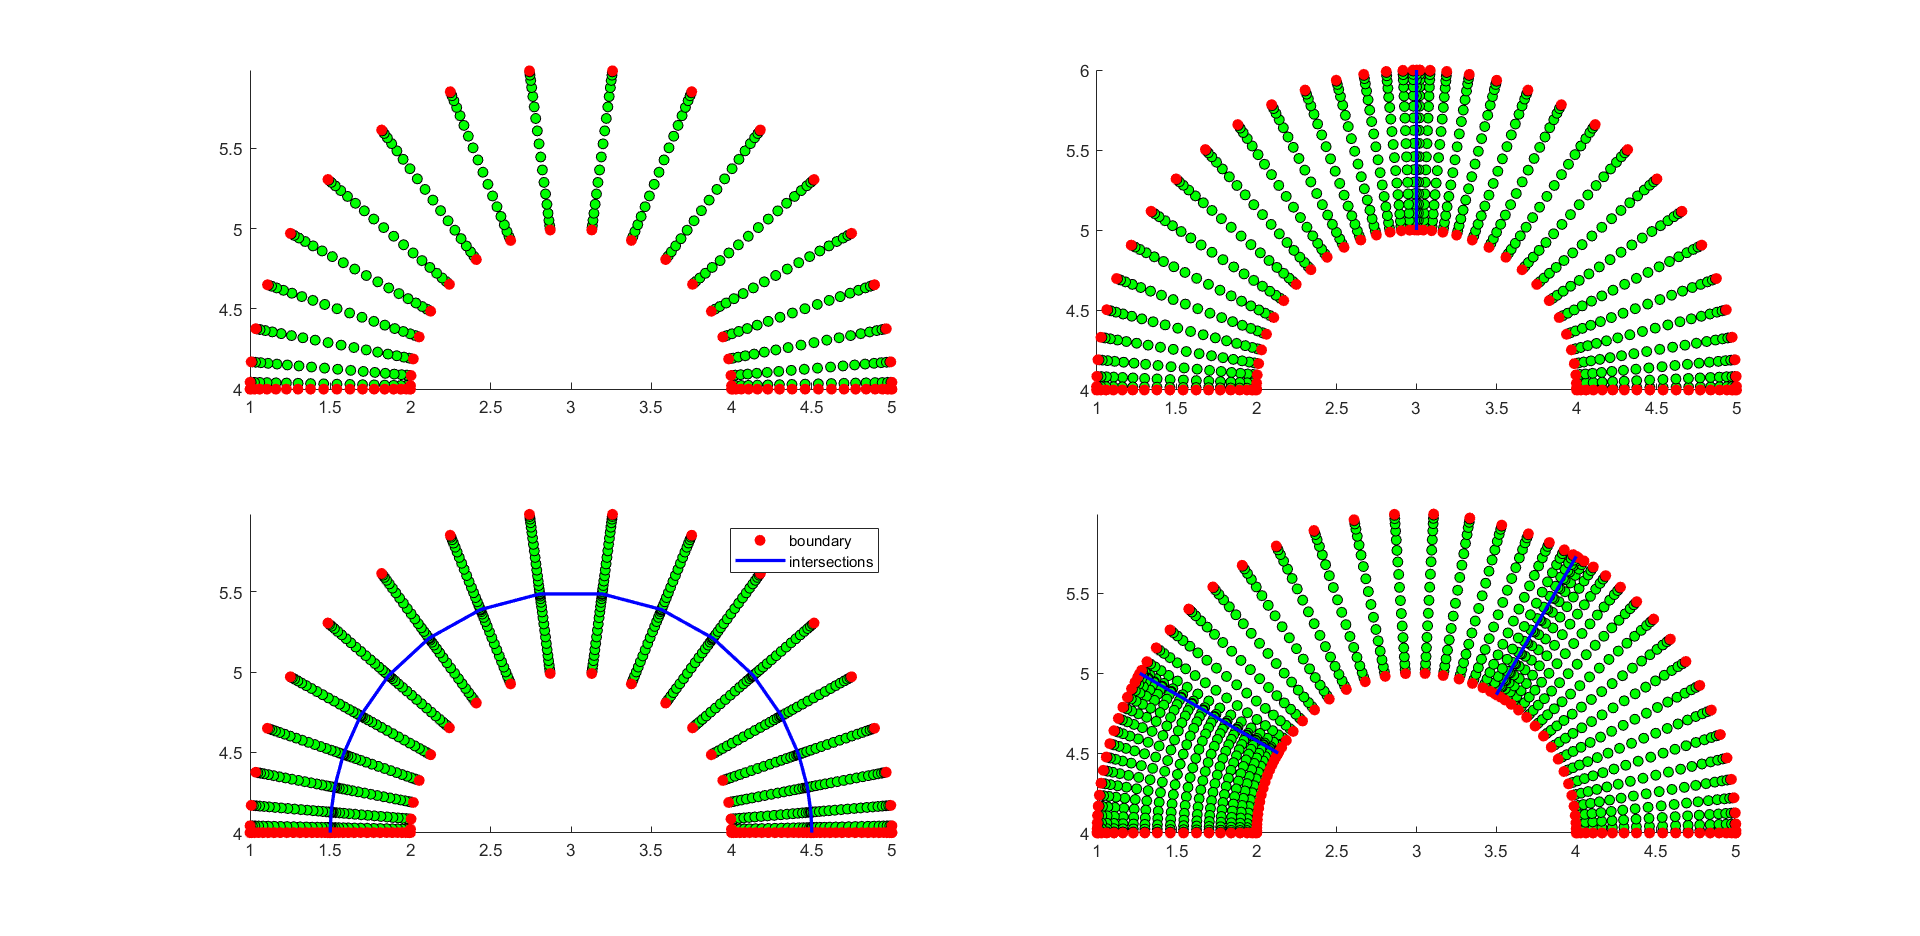
\includegraphics[scale=0.35]{WedgeSections.png}
	\caption{Different discretizations of the wedge.} 
	\label{F4}
\end{figure}

\begin{figure}[h]
	\centering
	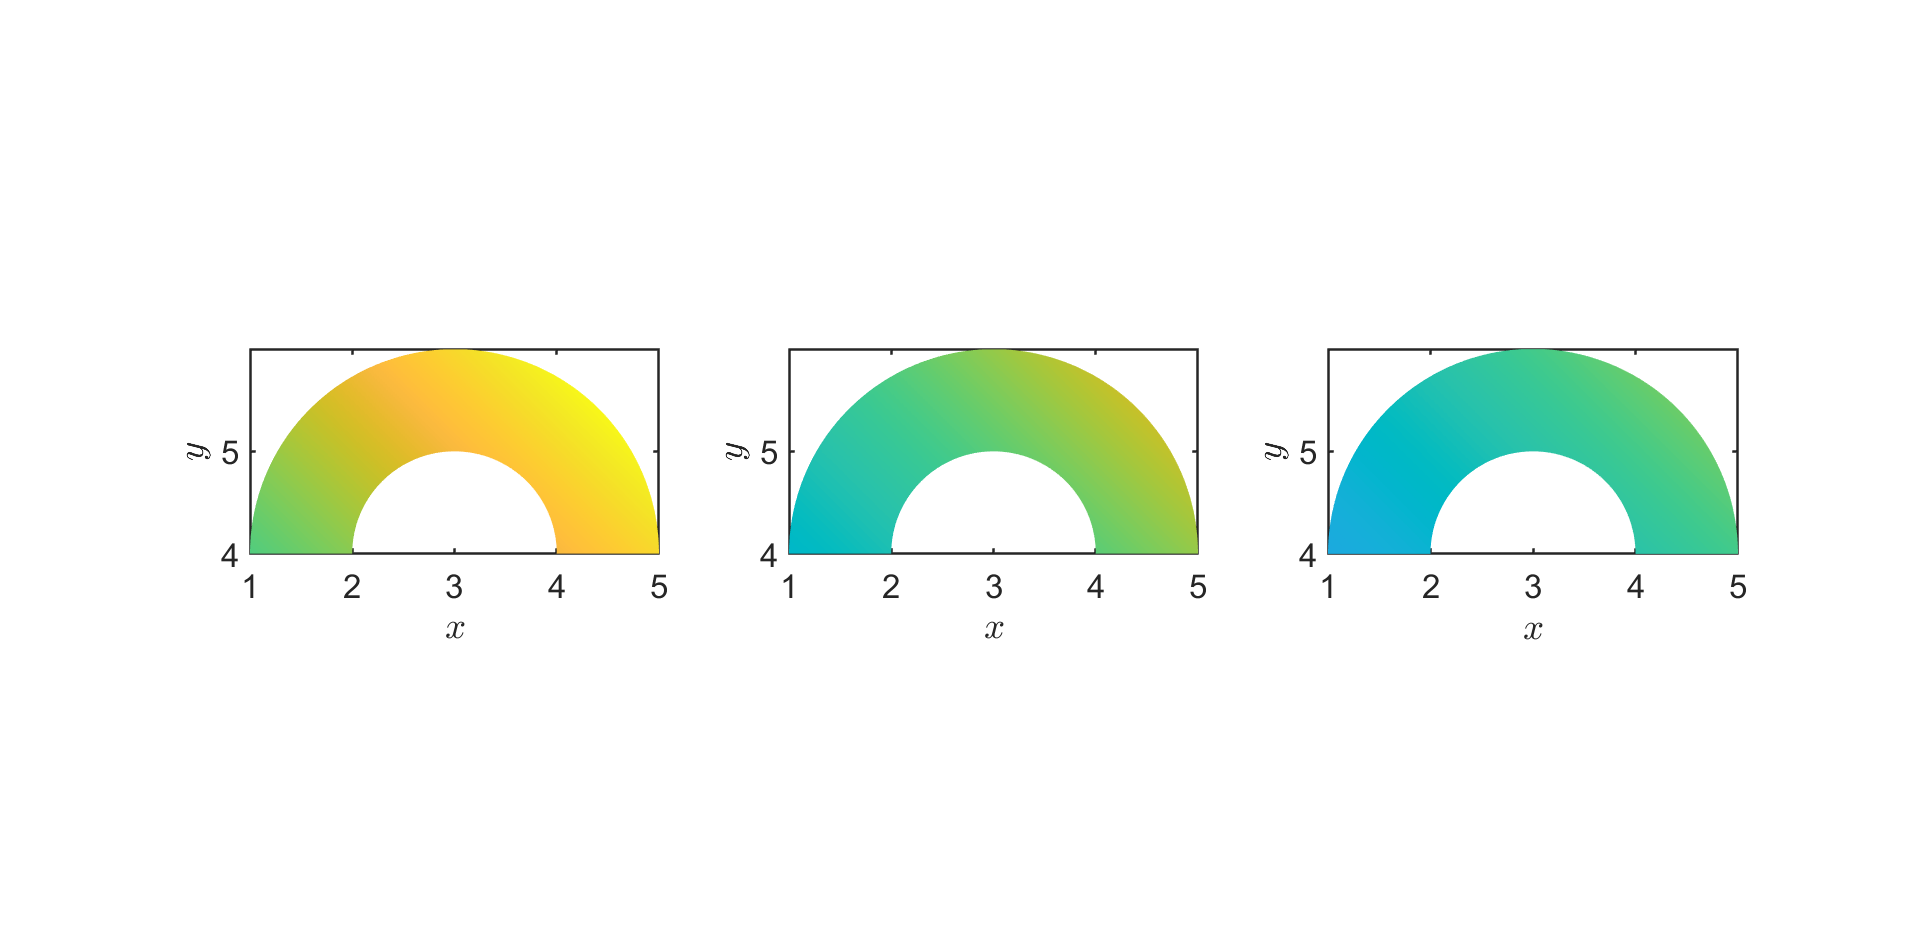
\includegraphics[scale=0.35]{wedgeEx.png}
	\caption{Exact solution on the wedge.} 
	\label{F5}
\end{figure}
\begin{table}
	\caption{Errors compared to exact solution for different discretization (into one, two and three shapes) of the wedge}
	\begin{tabular}{ ||c| c| c| c| c|| }
		\hline
		\hline
		& One Shape & Two Shapes (a) & Two Shapes (b)& Three Shapes\\ 
		\hline
		Abs. Error, $N =20$& $3.1141 \times 10^{-7}$ & $3.9526 \times 10^{-7}$ & $4.2335\times 10^{-7}$ & $4.4145\times 10^{-7}$\\  
		Rel. Error, $N =20$& $7.4762 \times 10^{-10}$& $7.5984 \times 10^{-10}$ &$7.4942 \times 10^{-10}$ &  $7.0897 \times 10^{-10}$\\
		Abs. Error, $N =30$& $ 2.7613\times 10^{-7}$ & $ 3.8484\times 10^{-7}$ & $3.892\times 10^{-7}$ & $4.3211\times 10^{-7}$ \\  
		Rel. Error, $N =30$ & $ 7.5178\times 10^{-10}$& $ 7.4375\times 10^{-10}$ &$7.5061\times 10^{-10}$ & $6.9683\times 10^{-10}$  \\
		\hline
		\hline
	\end{tabular}
	\label{Tab2:ErrorsExWedge}
\end{table}
Next the advection diffusion equation is solved on a multishape which is composed of four quadrilaterals, see Figure \ref{F6}. The absolute error for $N = 20$ on each shape as compared to the exact solution is $6.1246 \times 10^{-7}$ and the relative error is $1.3259 \times 10^{-9}$. 
\begin{figure}[h]
	\centering
	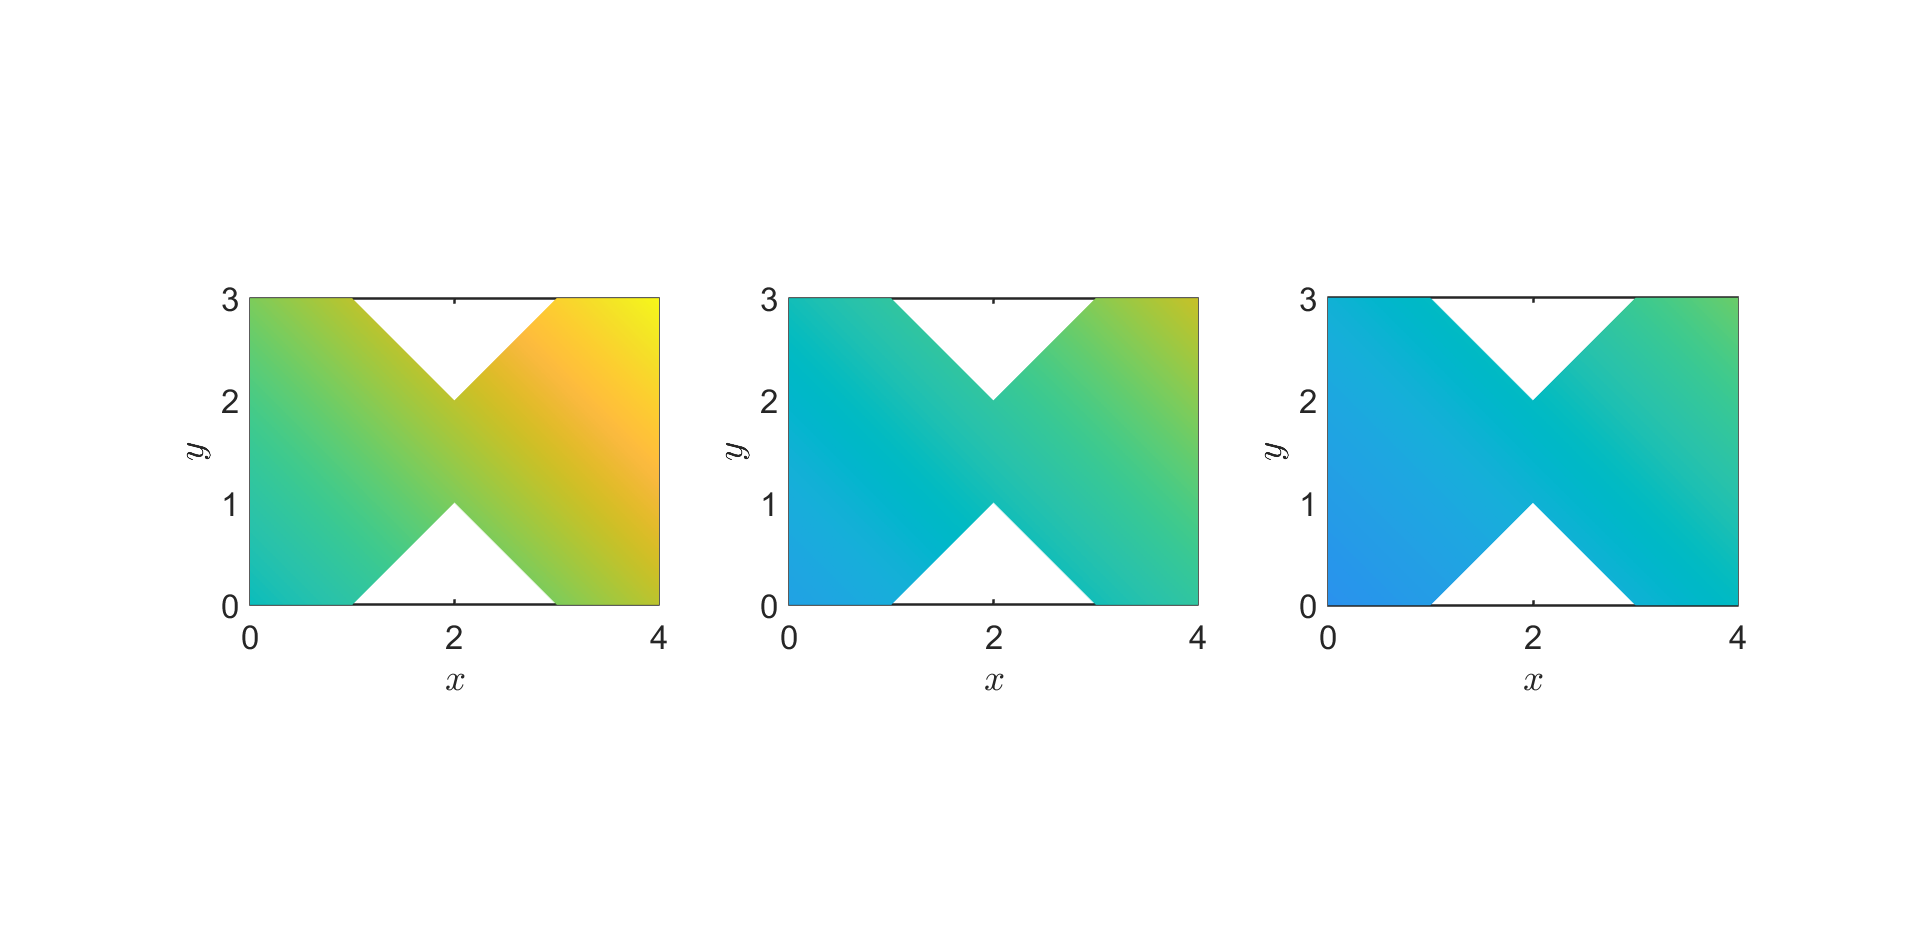
\includegraphics[scale=0.35]{example1.png}
	\caption{Example 1 multishape} 
	\label{F6}
\end{figure}
The same is done for a second example involving a wedge, see Figure \ref{F7}. The absolute error to the exact solution is $3.7239 \times 10^{-7}$ and the relative error is $8.9375 \times 10^{-10}$, when choosing $N= 20$ per shape. 

\begin{figure}[h]
	\centering
	\includegraphics[scale=0.35]{example2.png}
	\caption{Example 2 multishape} 
	\label{F7}
\end{figure}


\section{Forward Problems on multishapes}
We first consider a forward problem on the different discretizations of the box, see Figure \ref{F2}. We compare the error of the discretizations to the first box without discretization.
We choose the initial condition for $\rho$ to be
\begin{align*}
	\rho_0 = \exp(-2((y_1 - 0.7 )^2 + (y_2 - 0.2)^2))
\end{align*}
and impose a constant flow of strength $0.8$ acting upward.
We choose $N = 20$ and $N = 30$ as before. The errors are displayed in Table \ref{Tab3:ErrorsFWBox} and the result can be seen in Figure \ref{FFW1}. 

\begin{table}
	\caption{Errors (compared to whole box) for different discretization (into two, three and four shapes) of the box}
	\begin{tabular}{ ||c| c| c| c|| }
		\hline
		\hline
		& Two Shapes & Three Shapes & Four Shapes\\ 
		\hline
		Abs. Error, $N =20$& $0.0197$ & $0.0039$ & $0.01$ \\  
		Rel. Error, $N =20$& $0.0015$& $0.0005$ &$0.0007$ \\
		Abs. Error, $N =30$& $0.0103$ & $0.0021$ & $0.0053$  \\  
		Rel. Error, $N =30$ & $0.0005$& $0.0002$ &$0.0002$  \\
		\hline
		\hline
	\end{tabular}
	\label{Tab3:ErrorsFWBox}
\end{table}
\begin{figure}[h]
	\centering
	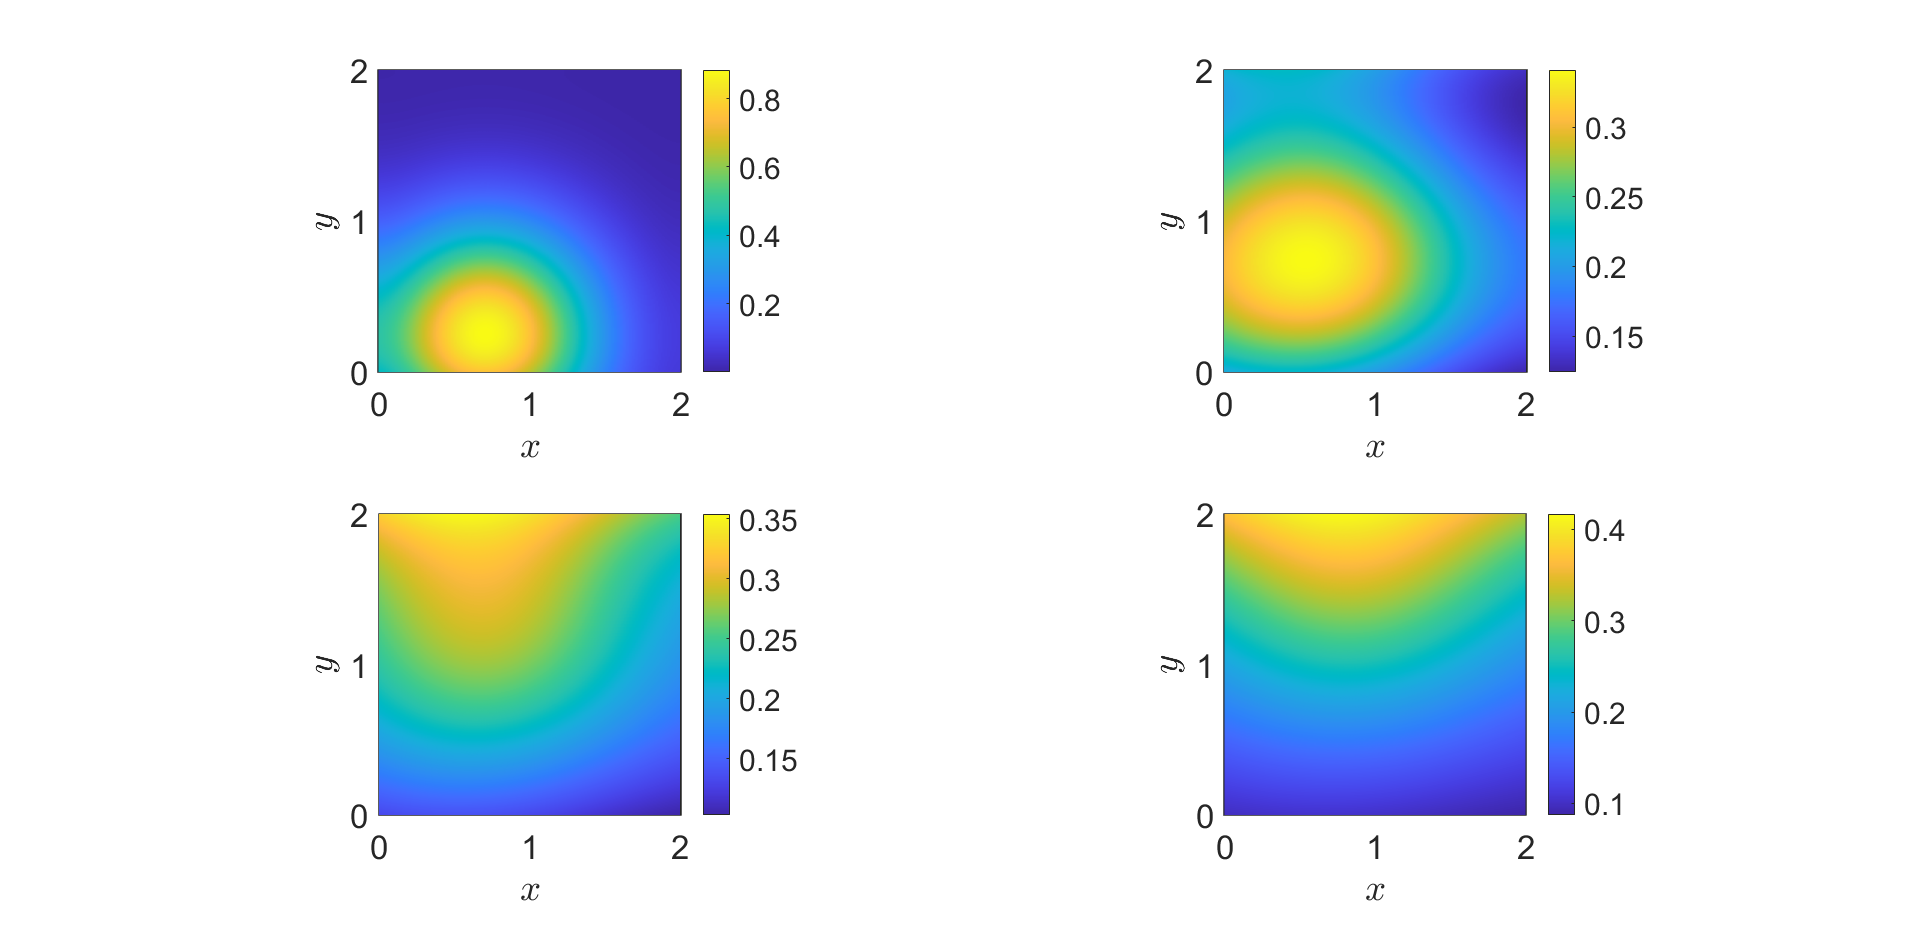
\includegraphics[scale=0.35]{FWBox.png}
	\caption{Forward Example on box discretizations} 
	\label{FFW1}
\end{figure}


We follow the same idea, but now consider the wedge discretizations, see Figure \ref{F4}. We choose the initial condition for $\rho$ to be
\begin{align*}
	\rho_0 = \exp(-2((y_1 - 1.5 )^2 + (y_2 - 4.5)^2))
\end{align*}
and impose a constant flow of strength $3$ acting from left to right, along the angular direction.
We choose $N = 20$ and $N = 30$. The errors are displayed in Table \ref{Tab4:ErrorsFWWedge} and the result can be seen in Figure \ref{FFW2}. 

\begin{table}
	\caption{Errors (compared to whole wedge) for different discretization (into two and three shapes) of the wedge}
	\begin{tabular}{ ||c| c| c| c|| }
		\hline
		\hline
		& Two Shapes (a) & Two Shapes (b) & Three Shapes\\ 
		\hline
		Abs. Error, $N =20$& $0.0386$ & $0.0076$ & $0.0693$ \\  
		Rel. Error, $N =20$& $0.0044$& $0.0007$ &$0.0047$ \\
		Abs. Error, $N =30$& $0.0215$ & $0.004$ & $0.0383$  \\  
		Rel. Error, $N =30$ & $0.0016$& $0.0002$ &$0.0017$  \\
		\hline
		\hline
	\end{tabular}
	\label{Tab4:ErrorsFWWedge}
\end{table}
\begin{figure}[h]
	\centering
	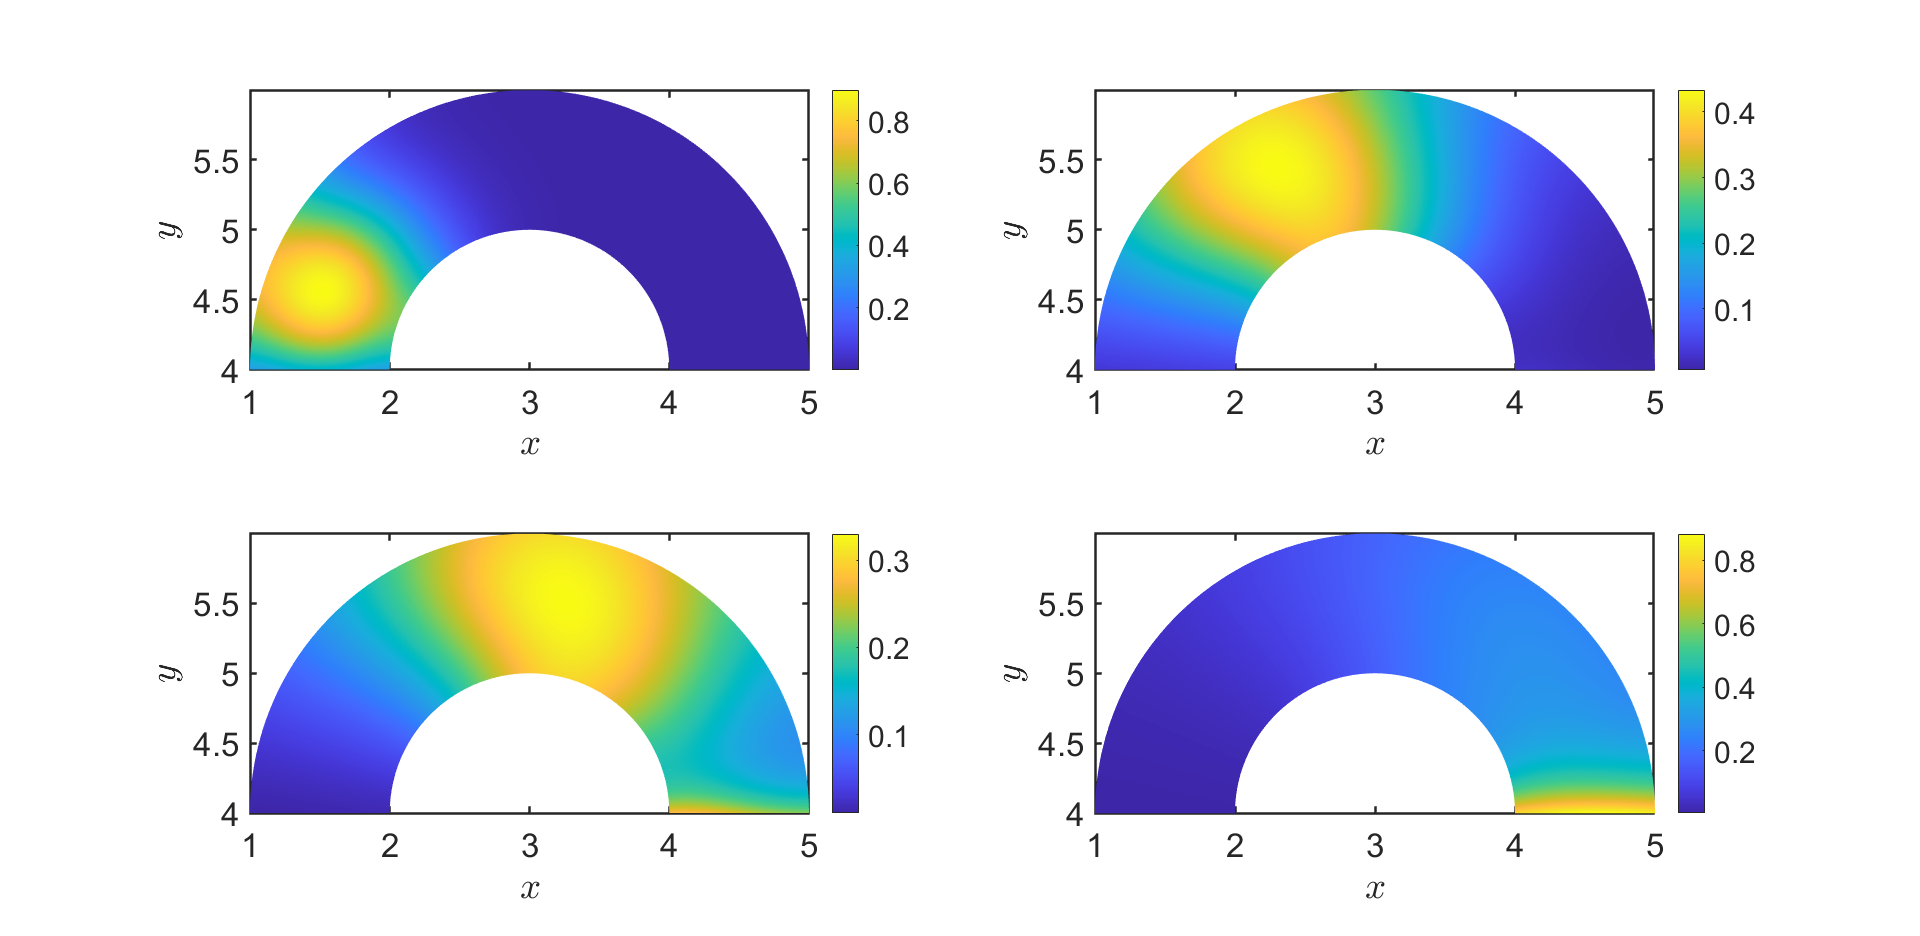
\includegraphics[scale=0.35]{FWWedge.png}
	\caption{Forward Example on wedge discretizations} 
	\label{FFW2}
\end{figure}



Finally, two multishape examples are shown, which are of interesting shapes.
The first of these examples is solving an advection diffusion problem on a multishape consisting of two quadrilaterals and two wedges, with constant velocity of strength ten. The initial condition for this problem is:
 \begin{align*}
 	\rho_0 = \exp( -2(y_1 -0.5)^2 - 2 (y_2 + 1)^2).
 \end{align*}
The result, evaluated for $N= 20$ on each shape, can be seen in Figure \ref{F8}.

\begin{figure}[h]
	\centering
	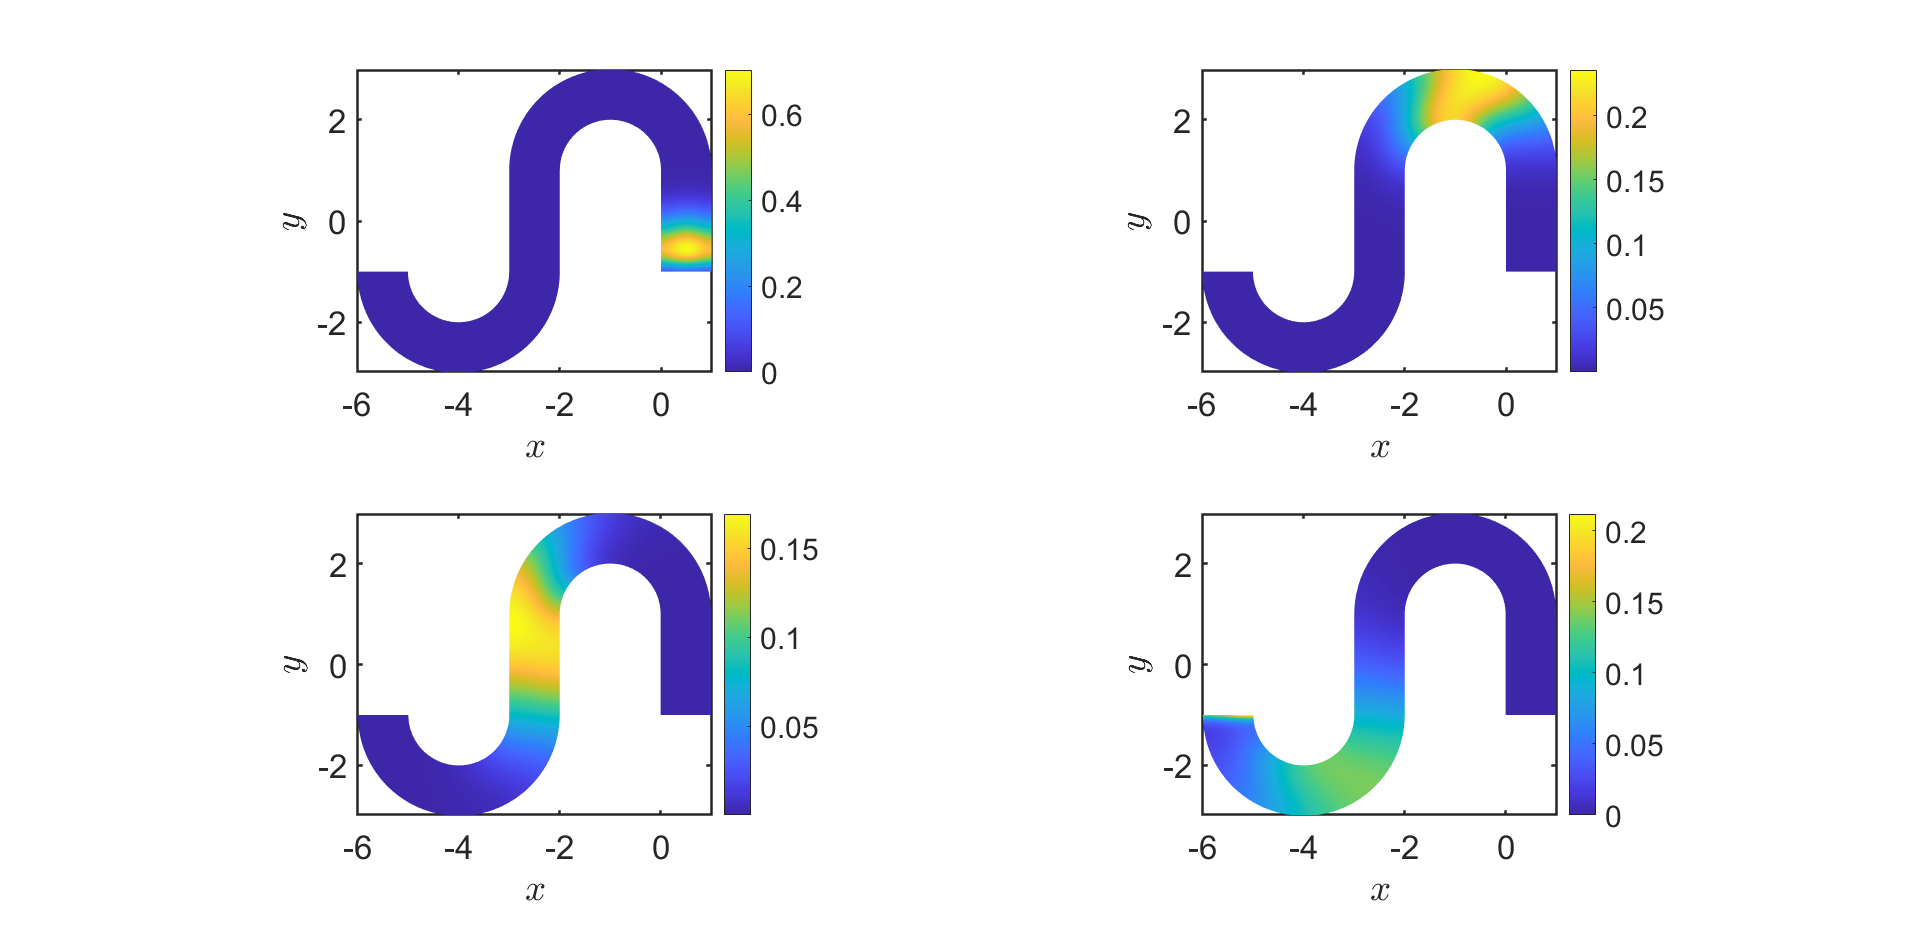
\includegraphics[scale=0.35]{ex1.png}
	\caption{Forward Problem 1, different colour scale for each plot to highlight particle mass location}
	\label{F8}
\end{figure}

In a second example, the velocity is of strength $5$ and the initial condition is:
 \begin{align*}
	\rho_0 = \exp( -2(y_1 -0.5)^2 - 2 (y_2 - 1.5)^2).
\end{align*}
The result, which is computed on a multishape made up of four quadrilaterals into a channel, can be seen in Figure \ref{F9}.

\begin{figure}[h]
	\centering
	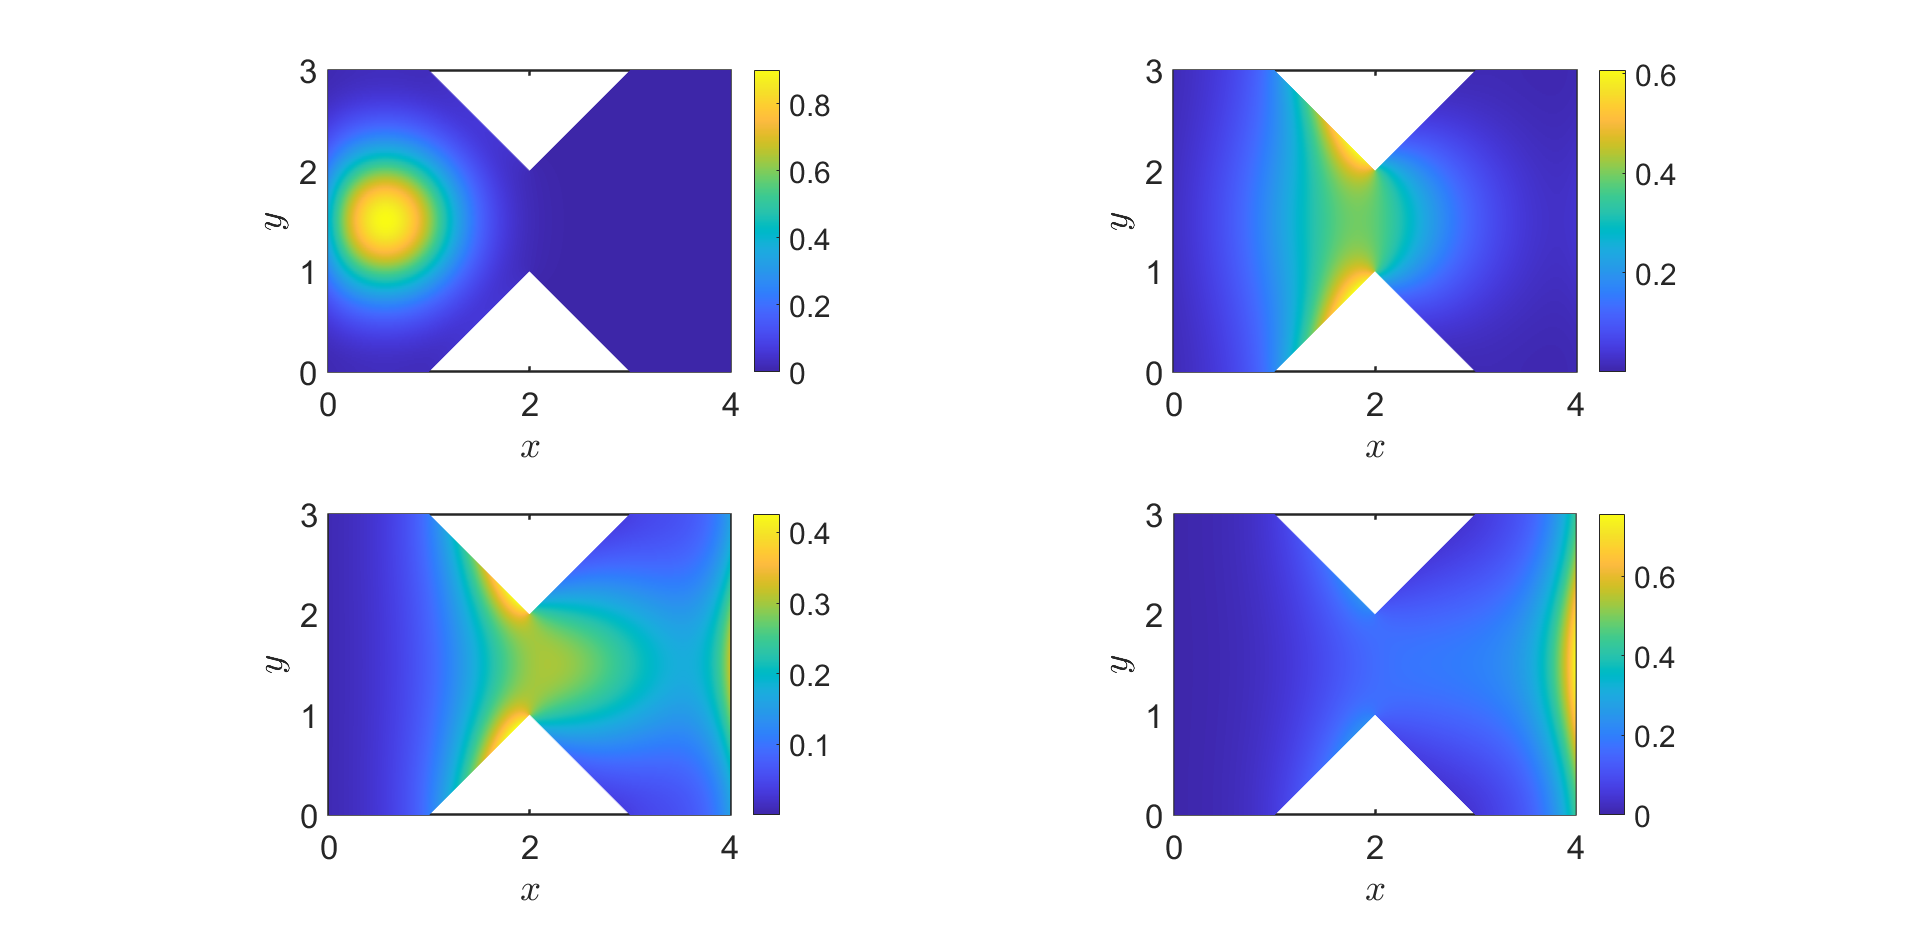
\includegraphics[scale=0.35]{ex2.png}
	\caption{Forward Problem 2, different colour scale for each plot to highlight particle mass location}
	\label{F9}
\end{figure}








\pagebreak	
\bibliography{GeneralBib}
\bibliographystyle{unsrt}
\end{document}